\chapter{Lecture 8 - Boiling Water Reactors and Supercritical Water Nuclear Reactors}
\label{ch:ch8}
\section{Objectives}
The objectives of this lecture are:
\begin{itemize}
\item Qualitative comparison between BWR and SCWR technologies
\item Quantitative example of SCWR energy conversion cycle
\item Practice analysis of complex Rankine cycles
\end{itemize}

\index{boiling water reactor}
\section{BWRs and Direct Cycles}
Early BWRs were built with the hopes of simplifying the system by having a direct steam cycle.  A schematic is shown in Figure \ref{fig:simple_BWR}.  
\begin{marginfigure}
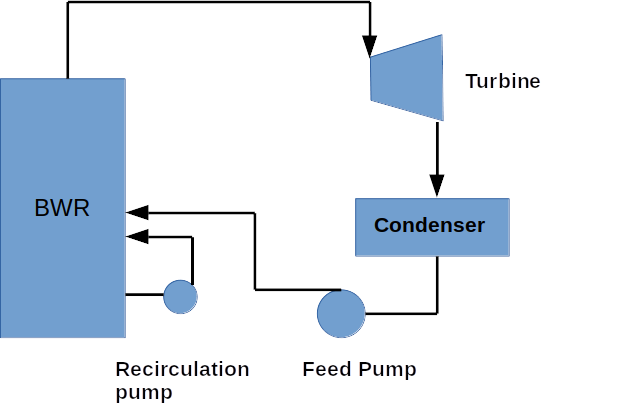
\includegraphics{simple_BWR.png}
\caption{Simplified BWR schematic.}
\label{fig:simple_BWR}
\end{marginfigure}
\newthought{Apart from the need} to contain radioactivity in the working fluid, this cycle is not, in principle, much different than the Rankine energy conversion cycle associated with a PWR.  Some of the advantages of a ``more simple'' direct cycle are offset by the lower power density achievable in the core of a BWR.\marginnote{\textbf{Note: }Typical core average power density for a BWR is 50 kW/l; roughly one half that achievable with a PWR.}  Most notably, the overall system for a given power output, is roughly as large as a PWR resulting in comparable construction costs; thus BWRs share one of the most significant problems with PWRs: high capital costs.

\section{Supercritical Water Nuclear Reactor}
\index{supercritical water reactor}
\newthought{One Gen IV concept} that has been developed with the aim of addressing the power-density issue with direct-cycle light water reactors is the Supercritical Water Nuclear reactor.\cite{tsiklauri2005supercritical} For this cycle, the water is maintained above the critical pressure throughout the heat-addition phase.  Good heat transfer can still be achieved without phase change and the prevention of bulk boiling prevents hydraulic instabilities that can be associated with BWR cores.  

\newthought{Additional notes are} provided in bullet-format:
\begin{itemize}
\item Elimination of phase change in the core eliminates the need for complex moisture separation equipment for fluid exiting the reactor core.  
\item Lack of phase change in the core also shifts the power distribution higher in the core relative to a typical BWR; the combination of this effect along with elimination of the moisture separation equipment favors locating the control rods at the top of the core.
\item Overall result is a smaller reactor pressure vessel and reduced containment size.
\end{itemize}
A schematic comparison of the size of a SCWR relative to competing PWR and BWR technologies is presented in Figure \ref{fig:SCWR_size}.
\begin{figure}
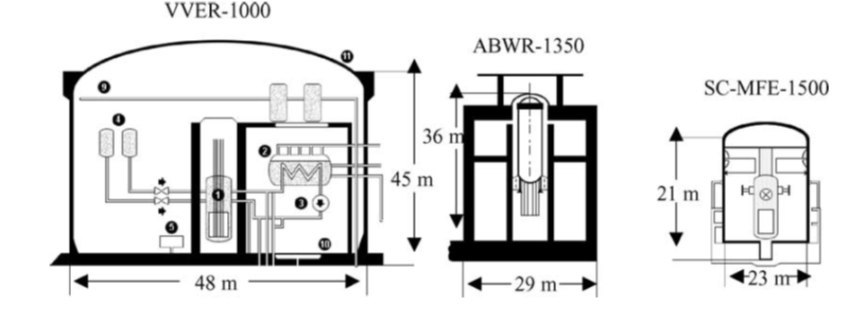
\includegraphics{BWR_SCWR_size_comparison.png}
\caption{Comparison of the size of containments for SC-MFE-1500, ABWR-1350 and VVER-1000.}
\label{fig:SCWR_size}
\end{figure}

\newthought{Even though moisture separation} equipment is not needed in the pressure vessel, there is a need for moisture separation equipment in the energy conversion cycle.  A temperature-entropy plot is drawn to scale in Figure \ref{fig:SCWR_TS}.  Even with very high core outlet temperature, when the supercritical fluid is expanded to low pressure moisture content of the working fluid becomes unacceptably high. Typical coal-fired steam plants operating at supercritical pressures deal with this issue by using one or more stages of reheat.  For nuclear powered systems, the steam piping arrangement necessary to use nuclear power for reheat can be impractical. For this cycle we will use additional moisture separation stages. 
\begin{marginfigure}
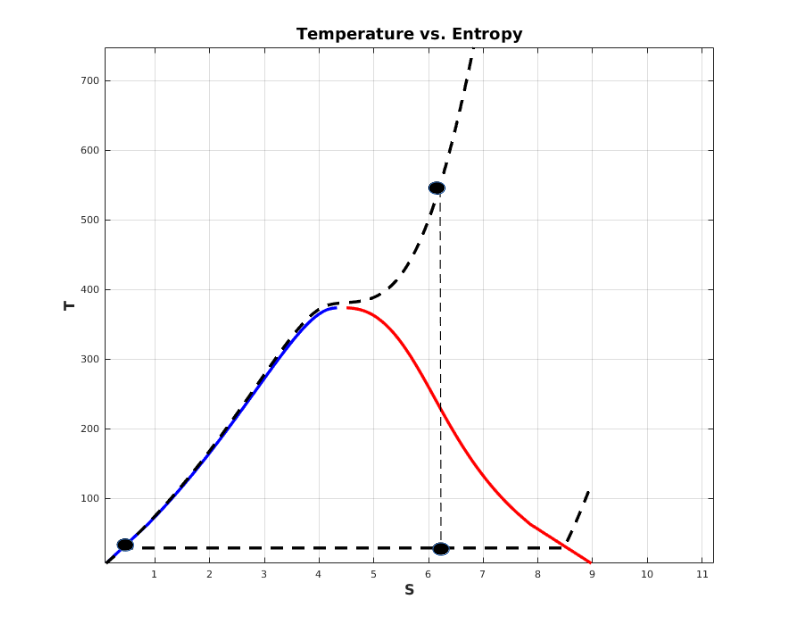
\includegraphics{SCWR_TS.png}
\caption{Temperature-entropy plot for SCWR drawn to scale.}
\label{fig:SCWR_TS}
\end{marginfigure}
A schematic of a potential SCWR energy conversion cycle is shown in Figure \ref{fig:SCWR_cycle}. Analysis of this cycle involves some complexity insofar as the flow fractions for each branch of the cycle needs to be determined but the details of such calculations are straight-forward.  Significant plant parameters are listed in Table \ref{tab:SCWR_params}.  Note the high thermal efficiency and high net specific work; with the moisture separators in use, the minimum turbine exhaust quality is more than 85 percent.  

\begin{margintable}
\begin{tabular}{cc}
\toprule
Parameter & Value \\
\midrule
$T_9$, $P_9$ & 550$^{\circ}$C, 24 MPa \\
HP Turbine Outlet Pressures & 8.9, 6, and 1 MPa \\
LP Turbine Outlet Pressures & 200 kPa, 4 kPa \\
$\eta_T$, $\eta_P$ & 0.9 and 0.88 \\
$w_{\text{net}}$ & 948 kJ/kg \\
Thermal Efficiency & 47.3 percent \\
\bottomrule
\end{tabular}
\caption{SCWR Parameters.}
\label{tab:SCWR_params}
\end{margintable}
\begin{figure}
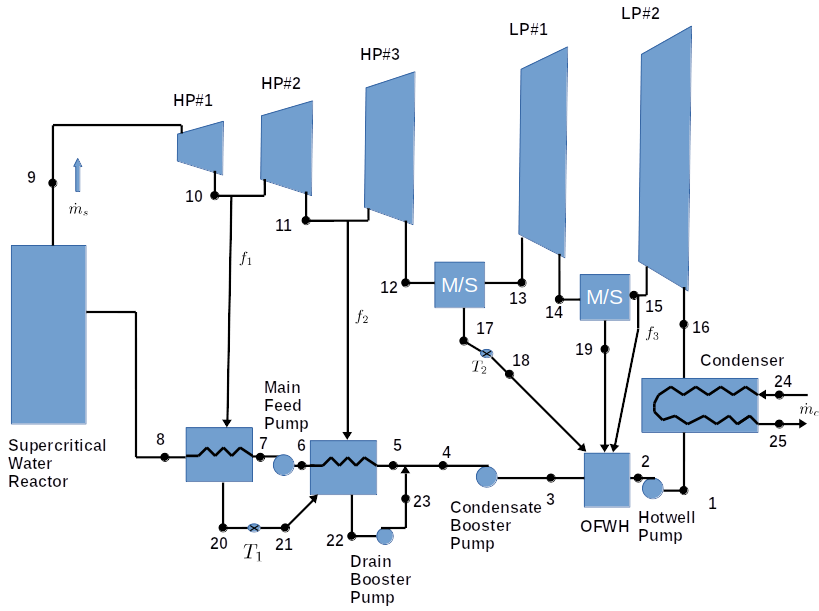
\includegraphics{SCWR_cycle.png}
\caption[][3cm]{SCWR power cycle with moisture separators. MATLAB code for a first-law analysis of this cycle is provided in the appendices.}
\label{fig:SCWR_cycle}
\end{figure}

\begin{example}
\textbf{Example calculations:} 
\begin{enumerate}
\item Write an expression for the specific work of Low Pressure Turbine \#2:

\emph{Answer:} $(h_{15}-h_{16})\left[(1-f_1)(1-f_2)x_{12}x_{14}(1-f_3) \right]$


\item Write an expression for the specific work of the Drain Booster Pump:

\emph{Answer:} $(h_{22}-h_{23})\left[f_1 + (1-f_1)f_2\right]$

\item Write an expression for the specific work of the Condensate Booster Pump:

\emph{Answer:} $(h_3 - h_4)[1 - (f_1 + (1-f_1)f_2)]$

\item Write an expression for the energy balance at the mixing point between the Condensate Booster Pump and CFWH \#2:

\emph{Answer:} $h_5 = [f_1+(1-f_1)f_2]h_{23} + [1-(f_1+(1-f_1)f_2]h_4$


\end{enumerate}
\end{example}



\begin{comment}
\begin{example}
\textbf{Challenge Problem:} Write an expression for the energy balance of the OFWH:
\emph{Answer:} 
\begin{multline*}
[1 - (f_1 + (1-f_1)f_2]h_3 = \\
(1-f_1)(1-f_2)x_{12}x_{14}(1-f_3)h_2 + \\
(1-f_1)(1-f_2)x_{12}x_{14}f_3h_{15} + \\
(1-f_1)(1-f_2)x_{12}(1-x_{14})h_{19} + \\
(1-f_1)(1-f_2)(1-x{12})h_{18} \\
\end{multline*}
\end{example}
\end{comment}


